\documentclass[tikz,border=10pt]{standalone}
\usepackage{tikz}
\usetikzlibrary{shapes.geometric, arrows.meta, positioning, calc, fit, backgrounds}
\usepackage{amsmath,amssymb}
\usepackage{xcolor}

% Unified Academic Color Palette
\definecolor{cInput}{RGB}{235, 248, 255}
\definecolor{bInput}{RGB}{49, 130, 206}

\definecolor{cTrans}{RGB}{240, 249, 255}
\definecolor{bTrans}{RGB}{43, 108, 176}

\definecolor{cGCN}{RGB}{230, 255, 250}
\definecolor{bGCN}{RGB}{49, 151, 149}

\definecolor{cRecurr}{RGB}{250, 245, 255}
\definecolor{bRecurr}{RGB}{128, 90, 213}

\definecolor{cHead}{RGB}{255, 245, 245}
\definecolor{bHead}{RGB}{229, 62, 62}

\definecolor{cFusion}{RGB}{254, 252, 191}
\definecolor{bFusion}{RGB}{214, 158, 46}

\definecolor{cGray}{RGB}{247, 250, 252}
\definecolor{bGray}{RGB}{160, 174, 192}

\definecolor{tDark}{RGB}{26, 32, 44}
\definecolor{tMuted}{RGB}{74, 85, 104}

\begin{document}
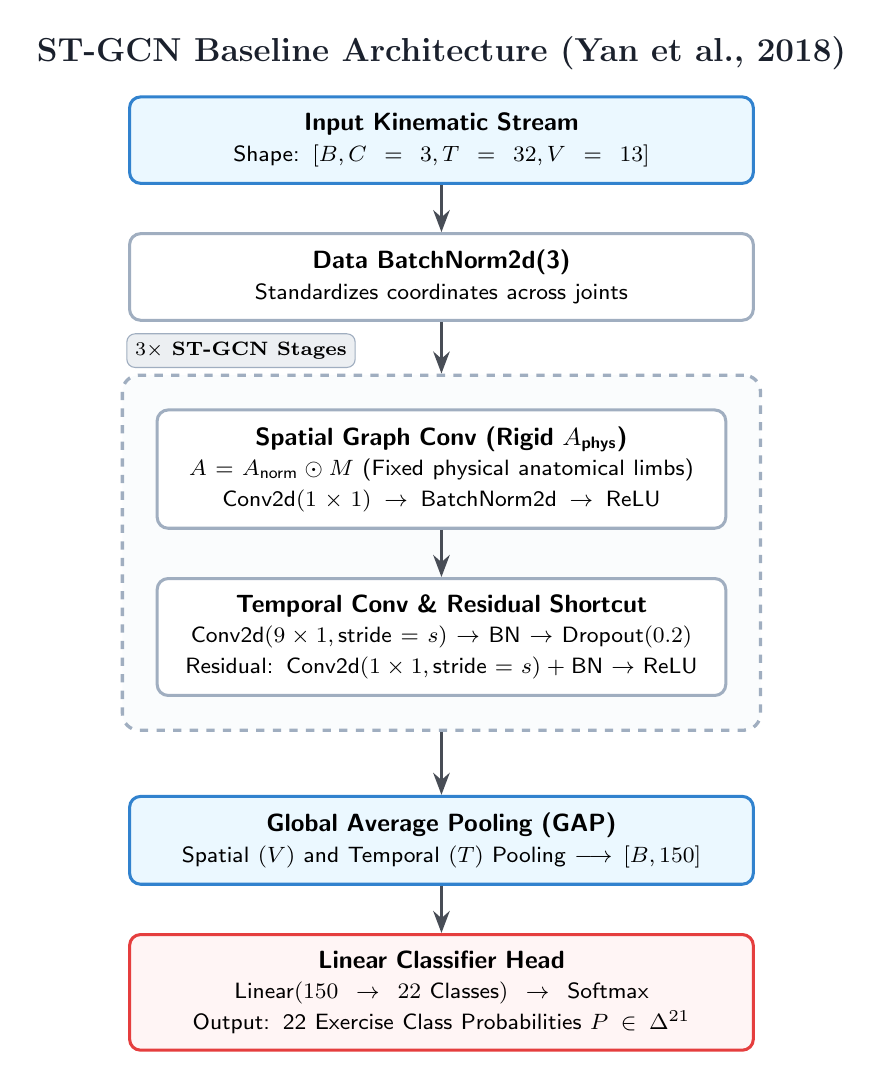
\begin{tikzpicture}[
    font=\sffamily\small,
    >=Stealth,
    node distance=0.6cm,
    block/.style={
        draw=#1,
        line width=1.1pt,
        rounded corners=4pt,
        align=center,
        inner sep=6pt
    },
    arrow/.style={->, line width=1.1pt, color=tDark!80}
]

\node[font=\bfseries\large, text=tDark] (title) at (0, 1.1) {ST-GCN Baseline Architecture (Yan et al., 2018)};

\node[block=bInput, fill=cInput, text width=7.5cm] (input) at (0, 0) {
    \textbf{Input Kinematic Stream}\\
    {\footnotesize Shape: $[B, C=3, T=32, V=13]$}
};

\node[block=bGray, fill=white, text width=7.5cm, below=of input] (bn) {
    \textbf{Data BatchNorm2d(3)}\\
    {\footnotesize Standardizes coordinates across joints}
};

% 3 Stages Container
\node[block=bGray, fill=white, text width=6.8cm, below=1.1cm of bn] (sgc) {
    \textbf{Spatial Graph Conv (Rigid $A_{\text{phys}}$)}\\
    {\footnotesize $A = A_{\text{norm}} \odot M$ (Fixed physical anatomical limbs)}\\
    {\footnotesize $\text{Conv2d}(1\times 1) \to \text{BatchNorm2d} \to \text{ReLU}$}
};

\node[block=bGray, fill=white, text width=6.8cm, below=0.6cm of sgc] (tcn) {
    \textbf{Temporal Conv \& Residual Shortcut}\\
    {\footnotesize $\text{Conv2d}(9\times 1, \text{stride}=s) \to \text{BN} \to \text{Dropout}(0.2)$}\\
    {\footnotesize Residual: $\text{Conv2d}(1\times 1, \text{stride}=s) + \text{BN} \to \text{ReLU}$}
};

\begin{scope}[on background layer]
    \node[draw=bGray, line width=1.2pt, dashed, rounded corners=6pt, fill=cGray!60,
          fit=(sgc)(tcn), inner sep=12pt] (cont) {};
    \node[anchor=south west, font=\bfseries\scriptsize, fill=bGray!20, draw=bGray, rounded corners=3pt, inner sep=3pt, xshift=2pt, yshift=2pt] at (cont.north west) {
        $3\times$ ST-GCN Stages
    };
\end{scope}

\node[block=bInput, fill=cInput, text width=7.5cm, below=0.8cm of cont] (gap) {
    \textbf{Global Average Pooling (GAP)}\\
    {\footnotesize Spatial $(V)$ and Temporal $(T)$ Pooling $\longrightarrow [B, 150]$}
};

\node[block=bHead, fill=cHead, text width=7.5cm, below=of gap] (head) {
    \textbf{Linear Classifier Head}\\
    {\footnotesize $\text{Linear}(150 \to 22 \text{ Classes}) \to \text{Softmax}$}\\
    {\footnotesize Output: 22 Exercise Class Probabilities $P \in \Delta^{21}$}
};

\draw[arrow] (input) -- (bn);
\draw[arrow] (bn) -- (cont);
\draw[arrow] (cont) -- (gap);
\draw[arrow] (gap) -- (head);
\draw[arrow] (sgc) -- (tcn);

\end{tikzpicture}
\end{document}
